\chapter{Results and Analysis} \label{results}
\hspace{\parindent}The statistical methods used for this thesis were one-way ANOVAs for each set of dependent measures \cite{ref_anova_1,ref_anova_2}, followed by a post-hoc analysis using Tukey's Honest Significant Difference (HSD) for multiple-compare \cite{ref_mult_compare}. The ranking system from the exit survey used the Friedman's test in conjunction with Tukey's HSD for a post-hoc analysis \cite{ref_friedmans}.

In addition, an n-way ANOVA was used on each set of variables for each keyboard with the participants' previous word-gesture experience as a factor. Surprisingly, there was no significant difference in mixed effects when using word-gesture experience as a factor, meaning participants who didn't have word-gesture experience performed as well as participants who did. This implies that interacting with word-gesture keyboards is intuitive (even applied to mid-air).

\section{Text-entry Rate} \label{results_text_entry_rate}
Participants reached a mean text-entry rate of 19.5 WPM ($SD = 3.0$) for the Touch Screen Keyboard, 17.1 WPM ($SD = 3.3$) for the Leap Surface Keyboard, 8.6 WPM ($SD = 1.9$) for the Leap Static-air Keyboard, 11.3 WPM ($SD = 2.0$) for the Leap Pinch-air Keyboard, 9.6 WPM ($SD = 2.3$) for the Predictive-air Keyboard, and 15.8 WPM ($SD = 2.2$) for the Leap Bimodal-air Keyboard. Figure~\ref{fig_textentry_mean} shows the mean text-entry rates for each keyboard interaction style.  It should be noted that the highest Bimodal-air text-entry rate, 20.7 WPM, was on par with the Touch Screen Keyboard text-entry rates. The Pinch-air keyboard, with a mean text-entry rate of 11.3 WPM, was consistent with the results from Vulture ($M = 11.8$) for participants' first session and no training \cite{ref_vulture}. Using a one-way ANOVA, a significant difference was detected between keyboard means ($F(5, 102) = 55.5017$, $p$-value $<$ 0.0001, $SD_{pooled} = 2.5$), prompting the use of Tukey's HSD with multiple-compare for further analysis.

\begin{figure}[!t]
	\centering
	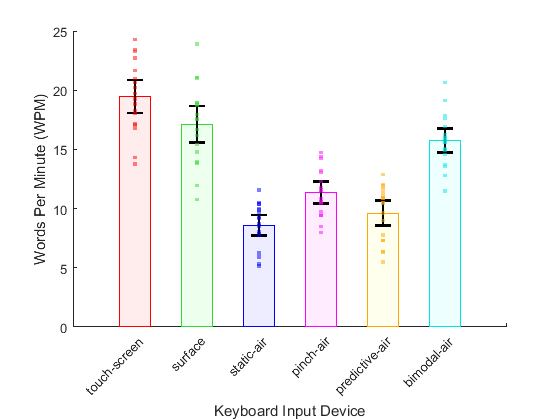
\includegraphics{Figures/fig_textentry_mean}
	\caption[Mean Text-entry Rates]{Mean Text-entry Rates for each keyboard with error bars showing 95\% confidence intervals.}
	\label{fig_textentry_mean}
\end{figure}

The multiple comparisons, seen in Table~\ref{textentry_multcompare}, revealed significant differences ($p$-values $<$ 0.001) in text-entry rates between the Touch Screen Keyboard and all mid-air keyboards. There were significant differences ($p$-values $<$ 0.0001) between the Leap Surface Keyboard and the Static-air, Pinch-air, and Predictive-air keyboards. There were also significant differences ($p$-values $<$ 0.0001) found between the Leap Bimodal-air and all other mid-air keyboards. Finally, there was a significant difference ($p$-value = 0.0170) found between the Pinch-air and Static-air keyboards.

Unfortunately, no mid-air keyboards were able to achieve text-entry rates as fast as the Touch Screen Keyboard and were significantly slower. However, the Bimodal-air keyboard reached a mean text-entry rate of 15.8 WPM without repeated sessions or training, indicating promising results. With repeated sessions, as in Vulture \cite{ref_vulture}, the Bimodal Keyboard is expected to increase in performance by approximately 75\%. The increase is expected to be even greater (approximately 238\%) when training for single short phrases, reaching speeds sufficiently high enough to compete with touch-based keyboards and surpass pinching as a means of mid-air word-gesturing.

Both the Static-air and Predictive-air keyboards underperformed, though the Predictive-air keyboard achieved marginally better results. These results were expected since adding the 3rd-dimension as a means of interaction further increased keyboard complexity and the mental coupling required between gestures in the motor-space and feedback on the display \cite{ref_vulture,ref_stimulus_response_compatibility}. It was interesting to see how well the Leap Surface Keyboard performed since it had an identical implementation as the Leap Static-air Keyboard, only differing in where the interaction plane was projected. This implies that visually representing the Leap Static-air keyboard in 3-dimensional space using augmented reality might have the same results due to the decreased decoupling between the motor space and display space.

\subsection{Text-entry Rate Modified-shortest}
Participants reached a mean text-entry rate of 19.7 WPM ($SD = 2.9$) for the Touch Screen Keyboard, 17.3 WPM ($SD = 3.3$) for the Leap Surface Keyboard, 8.8 WPM ($SD = 1.9$) for the Leap Static-air Keyboard, 11.6 WPM ($SD = 2.1$) for the Leap Pinch-air Keyboard, 9.9 WPM ($SD = 2.3$) for the Predictive-air Keyboard, and 15.9 WPM ($SD = 2.2$) for the Leap Bimodal-air Keyboard. Figure~\ref{fig_textentry_short_mean} shows the mean text-entry rates for each keyboard interaction style using the shortest-transcribed modification. Using a one-way ANOVA, a significant difference was detected between keyboard means ($F(5, 102) = 54.6430$, $p$-value $<$ 0.0001, $SD_{pooled} = 2.5$), prompting the use of Tukey's HSD with multiple-compare for further analysis.

\begin{figure}[!t]
	\centering
	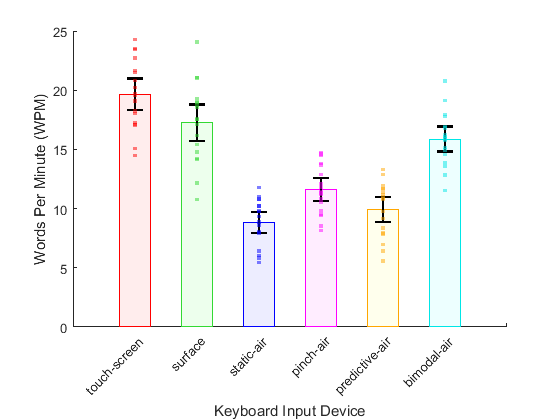
\includegraphics{Figures/fig_textentry_short_mean}
	\caption[Mean Text-entry Rates for Modified-shortest]{Mean Text-entry Rates using the shortest-transcribed modification for each keyboard with error bars showing 95\% confidence intervals.}
	\label{fig_textentry_short_mean}
\end{figure}

The multiple comparisons, seen in Table~\ref{textentry_short_multcompare}, revealed significant differences ($p$-values $<$ 0.001) in text-entry rates between the Touch Screen Keyboard and all mid-air keyboards. There were significant differences ($p$-values $<$ 0.0001) between the Leap Surface Keyboard and the Static-air, Pinch-air, and Predictive-air keyboards. There were also significant differences ($p$-values $<$ 0.0001) found between the Leap Bimodal-air and all other mid-air keyboards. The highest Bimodal-air text-entry rates were on par with the Touch Screen Keyboard. Finally, there was a significant difference ($p$-value = 0.0148) found between the Pinch-air and Static-air keyboards.

The results from using the shortest-transcribed modification were marginally better than those without, implying that errors were more likely corrected while gesturing the words rather than after having completed the gesture. The cases where errors were made while still entering all required letters seem to have had very little impact on the duration it took to complete words.

\section{Error Rate}

\subsection{Minimum Word Distance}
Participants reached a mean MWD of 13.0\% ($SD = 13.4$) for the Touch Screen Keyboard, 18.9\% ($SD = 14.0$) for the Leap Surface Keyboard, 56.7\% ($SD = 19.4$) for the Leap Static-air Keyboard, 34.4\% ($SD = 19.4$) for the Leap Pinch-air Keyboard, 48.9\% ($SD = 25.2$) for the Predictive-air Keyboard, and 20.4\% ($SD = 16.9$) for the Leap Bimodal-air Keyboard. Figure~\ref{fig_MWD_mean} shows the mean Minimum Word Distance for each keyboard interaction style. Using a one-way ANOVA, a significant difference was detected between keyboard means ($F(5, 102) = 16.5496$, $p$-value $<$ 0.0001, $SD_{pooled} = 18.5$), prompting the use of Tukey's HSD with multiple-compare for further analysis.

\begin{figure}[!t]
	\centering
	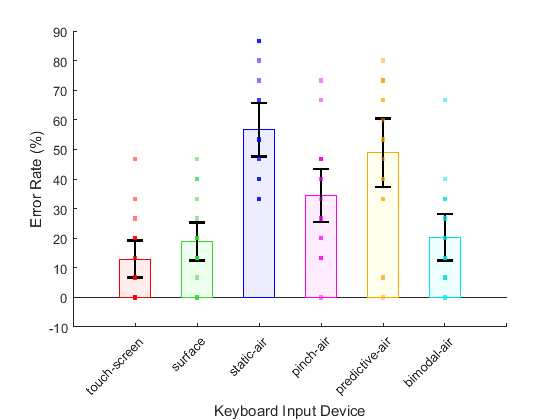
\includegraphics{Figures/fig_MWD_mean}
	\caption[Mean Minimum Word Distance]{Mean Minimum Word Distance for each keyboard with error bars showing 95\% confidence intervals.}
	\label{fig_MWD_mean}
\end{figure}

The multiple comparisons, seen in Table~\ref{MWD_multcompare}, revealed significant differences ($p$-values $<$ 0.01) in Minimum Word Distance between the Touch Screen Keyboard and the Leap Static-air, Pinch-air, and Predictive-air keyboards. There were significant differences ($p$-values $<$ 0.0001) between the Leap Surface Keyboard and the Static-air and Predictive-air keyboards. There were also significant differences ($p$-values $<$ 0.001) found between the Leap Bimodal-air and the Static-air and Predictive-air keyboards. There was finally a significant difference ($p$-value = 0.0062) found between the Leap Pinch-air and Static-air keyboards.

The error rates here were much higher than those seen in Vulture for Pinch or Touch \cite{ref_vulture} because this was a modified version of MWD. Since participants were required to fix errors, the MWD from Vulture would have seen error rates of 0\%. Instead, if any errors were detected during the typing process, whether it be from device detection issues or the participant going for the wrong letter, the word was counted as erroneous. This representation of MWD showed how many words needed correcting for any reason.

The Static-air and Predictive-air keyboards underperformed, as expected, due to the increased decoupling and the added complexity of working with the 3rd-dimension. The Leap Bimodal-air Keyboard was significantly less erroneous than the Static-air and Predictive-air keyboards and was not significantly different from the Touch Screen Keyboard, implying that removing the 3rd-dimension significantly reduces the effects of decoupling on hand-eye coordination efforts. Again, the Leap Surface was on par with the Touch Screen keyboard, suggesting that with augmented reality the Static-air Keyboard could see a significant improvement in performance in all areas.

\subsubsection{MWD modified-shortest}
Participants reached a mean MWD of 6.3\% ($SD = 9.0$) for the Touch Screen Keyboard, 6.3\% ($SD = 6.3$) for the Leap Surface Keyboard, 25.6\% ($SD = 20.7$) for the Leap Static-air Keyboard, 20.0\% ($SD = 11.2$) for the Leap Pinch-air Keyboard, 26.0\% ($SD = 16.6$) for the Predictive-air Keyboard, and 10.0\% ($SD = 11.7$) for the Leap Bimodal-air Keyboard. Figure~\ref{fig_MWD_short_mean} shows the mean Minimum Word Distance with the shortest-transcribed modification for each keyboard interaction style. Using a one-way ANOVA, a significant difference was detected between keyboard means ($F(5, 102) = 8.5172$, $p$-value $<$ 0.0001, $SD_{pooled} = 13.5$), prompting the use of Tukey's HSD with multiple-compare for further analysis.

\begin{figure}[!t]
	\centering
	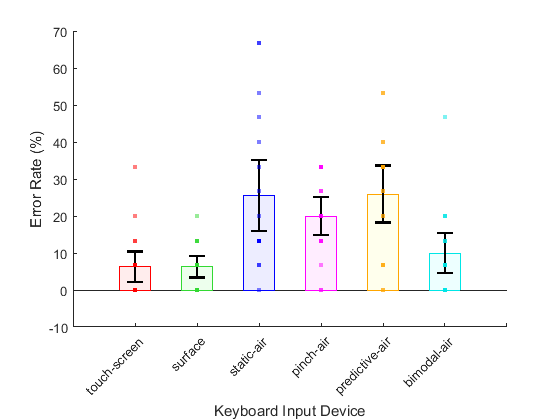
\includegraphics{Figures/fig_MWD_short_mean}
	\caption[Mean Minimum Word Distance for Modified-shortest]{Mean Minimum Word Distance using the shortest-transcribed modification for each keyboard with error bars showing 95\% confidence intervals.}
	\label{fig_MWD_short_mean}
\end{figure}

The multiple comparisons, seen in Table~\ref{MWD_short_multcompare}, revealed significant differences ($p$-values $<$ 0.05) in Minimum Word Distance with the shortest-transcribed modification between the Touch Screen Keyboard and the Leap Static-air, Pinch-air, and Predictive-air keyboards. There were significant differences ($p$-values $<$ 0.05) between the Leap Surface Keyboard and the Leap Static-air, Pinch-air, and Predictive-air keyboards. There were also significant differences ($p$-values $<$ 0.01) found between the Leap Bimodal-air and the Static-air and Predictive-air keyboards.

The substantial reductions in MWD error rates when using the shortest-transcribed modification, nearly 50\% reduction for all keyboards, indicated that many participants seemed to be making errors after entering all of the required letters for a gestured word. This may imply situations like Example 4 from Table~\ref{shortest_transcribed}, where participants were typing the wrong word, such as ``fired'' compared to ``fire''. However, for all Leap Motion-based keyboards, the more likely implication is that many participants made errors on exiting the interaction plane. This kind of error was observed often and was thought to be heavily influenced by participants pulling their hands away from the interaction plane in an arcing motion, especially for participants who were resting their arms. Figure~\ref{arcing_motion} details this arcing motion. It is expected that a word-recognition implementation of the word-gesture keyboards would see even lower error rates closer to those found in Vulture \cite{ref_vulture}, implying that the pseudo-implementation of the word-gesture keyboards was less robust and more sensitive to deviations in a word's gesture-shape than traditional word-gesture keyboards implemented with word-recognition.

\begin{figure}[!t]
	\centering
	\begin{minipage}[t]{2.5in}
		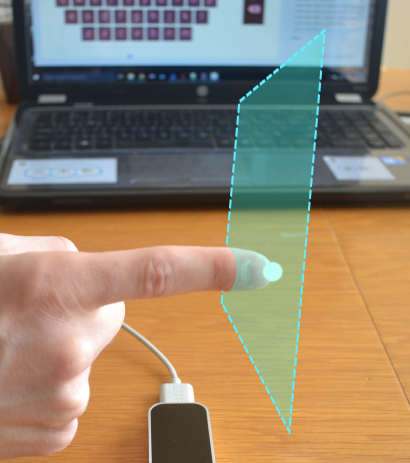
\includegraphics[width=2.5in]{Figures/fig_arc_down}
		\subcaption{Pressing Final Key}
	\end{minipage}
	\begin{minipage}[t]{2.5in}
		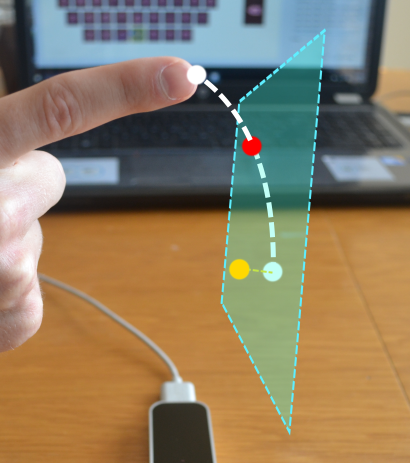
\includegraphics[width=2.5in]{Figures/fig_arc_up}
		\subcaption{Removing Hand From Plane}
	\end{minipage}
	\caption[Arcing Motion]{Examples of how the natural arcing motion generates erroneous input for 3-dimensional interactions. (a) shows the user pressing the final key; and (b) shows the intended release in \textit{yellow} and the detected release in \textit{red}.}
	\label{arcing_motion}
\end{figure}

\subsection{Keystrokes Per Character}
Participants reached a mean KSPC of 1.2 keystrokes per character ($SD = 0.18$) for the Touch Screen Keyboard, 1.4 keystrokes per character  ($SD = 0.38$) for the Leap Surface Keyboard, 2.0 keystrokes per character ($SD = 0.79$) for the Leap Static-air Keyboard, 1.6 keystrokes per character ($SD = 0.42$) for the Leap Pinch-air Keyboard, 1.9 keystrokes per character ($SD = 0.64$) for the Predictive-air Keyboard, and 1.2 keystrokes per character ($SD = 0.18$) for the Leap Bimodal-air Keyboard. Figure~\ref{fig_KSPC_mean} shows the mean Keystrokes Per Character for each keyboard interaction style. Using a one-way ANOVA, a significant difference was detected between keyboard means ($F(5, 102) = 9.8827$, $p$-value $<$ 0.0001, $SD_{pooled} = 0.49$), prompting the use of Tukey's HSD with multiple-compare for further analysis.

\begin{figure}[!t]
	\centering
	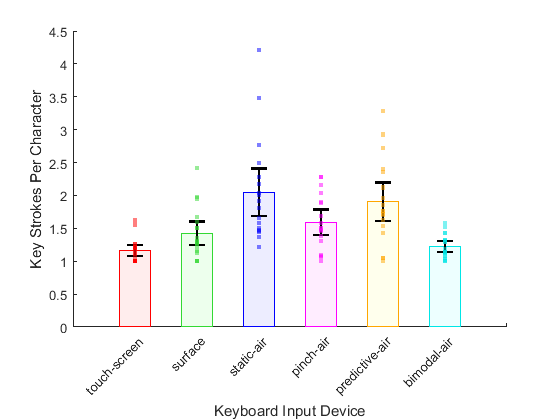
\includegraphics{Figures/fig_KSPC_mean}
	\caption[Mean Keystrokes Per Character]{Mean Keystrokes Per Character for each keyboard with error bars showing 95\% confidence intervals.}
	\label{fig_KSPC_mean}
\end{figure}

The multiple comparisons, seen in Table~\ref{KSPC_multcompare}, revealed significant differences ($p$-values $<$ 0.001) in Keystrokes Per Character between the Touch Screen Keyboard and the Leap Static-air and Predictive-air keyboards. There were significant differences ($p$-values $<$ 0.05) between the Leap Surface Keyboard and the Static-air and Predictive-air keyboards. There were also significant differences ($p$-values $<$ 0.01) found between the Leap Bimodal-air and the Static-air and Predictive-air keyboards.

Keystrokes Per Character was useful when analyzing the pseudo implementation of the word-gesture keyboards because words were constructed at the character level, rather than at the word level as with word-recognition. With KSPC, if words were input without any detected errors, then a KSPC of 1.0 keystrokes would be expected. This metric helps show the rate at which extra erroneous characters were produced for each keyboard. For example, the KSPC of the Static-air keyboard was 2.0 keystrokes, meaning 100\% more interactions were produced than required to gesture the words successfully. As before, the Static-air and Predictive-air keyboard performances were underwhelming, and the Bimodal-air performed on par with the Touch Screen and Leap Surface keyboards. The Pinch-air performed somewhere in between the other Leap Motion-based keyboards. As these means continue to show, a trend was developing in the dependent measures between the keyboards and was expected to hold for all other variables.

\subsubsection{KSPC modified-shortest}
Participants reached a mean KSPC of 1.1 keystrokes per character ($SD = 0.14$) for the Touch Screen Keyboard, 1.3 keystrokes per character ($SD = 0.27$) for the Leap Surface Keyboard, 1.7 keystrokes per character ($SD = 0.48$) for the Leap Static-air Keyboard, 1.4 keystrokes per character ($SD = 0.31$) for the Leap Pinch-air Keyboard, 1.7 keystrokes per character ($SD = 0.43$) for the Predictive-air Keyboard, and 1.1 keystrokes per character ($SD = 0.15$) for the Leap Bimodal-air Keyboard. Figure~\ref{fig_KSPC_short_mean} shows the mean Keystrokes Per Character with the shortest-transcribed modification for each keyboard interaction style. Using a one-way ANOVA, a significant difference was detected between keyboard means ($F(5, 102) = 11.5949$, $p$-value $<$ 0.0001, $SD_{pooled} = 0.32$), prompting the use of Tukey's HSD with multiple-compare for further analysis.

\begin{figure}[!t]
	\centering
	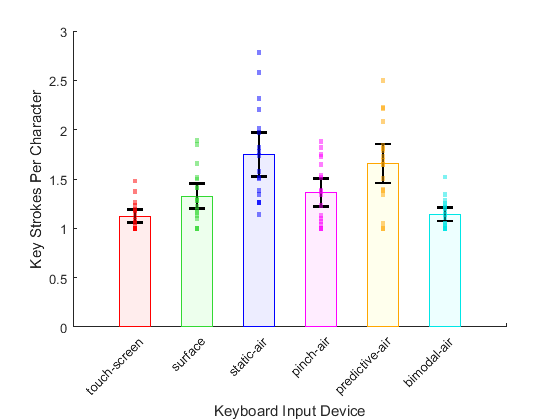
\includegraphics{Figures/fig_KSPC_short_mean}
	\caption[Mean Keystrokes Per Character for Modified-shortest]{Mean Keystrokes Per Character using the shortest-transcribed modification for each keyboard with error bars showing 95\% confidence intervals.}
	\label{fig_KSPC_short_mean}
\end{figure}

The multiple comparisons, seen in Table~\ref{KSPC_short_multcompare}, revealed significant differences ($p$-values $<$ 0.0001) in Keystrokes Per Character with the shortest-transcribed modification between the Touch Screen Keyboard and the Leap Static-air and Predictive-air keyboards. There were significant differences ($p$-values $<$ 0.05) between the Leap Surface Keyboard and the Leap Static-air and Predictive-air keyboards. There were also significant differences ($p$-values $<$ 0.001) found between the Leap Bimodal-air Keyboard and the Static-air and Predictive-air keyboards. Finally there was a significant difference ($p$-value = 0.0072) between the Pinch-air and Static-air keyboards.

As with MWD, KSPC saw huge improvements with the shortest-transcribed modification, especially for Leap Motion-based keyboards. This reaffirmed that a large number of errors were produced during exiting the interaction plane.

\subsection{Minimum String Distance}

\subsubsection{MSD modified-shortest}
Participants reached a mean MSD of 1.6\% ($SD = 2.4$) for the Touch Screen Keyboard, 2.2\% ($SD = 2.4$) for the Leap Surface Keyboard, 6.4\% ($SD = 5.0$) for the Leap Static-air Keyboard, 5.1\% ($SD = 3.1$) for the Leap Pinch-air Keyboard, 5.4\% ($SD = 3.3$) for the Predictive-air Keyboard, and 2.5\% ($SD = 2.6$) for the Leap Bimodal-air Keyboard. Figure~\ref{fig_MSD_short_mean} shows the mean Minimum String Distance with the shortest-transcribed modification for each keyboard interaction style. Using a one-way ANOVA, a significant difference was detected between keyboard means ($F(5, 102) = 6.8688$, $p$-value $<$ 0.0001, $SD_{pooled} = 3.3$), prompting the use of Tukey's HSD with multiple-compare for further analysis.

\begin{figure}[!t]
	\centering
	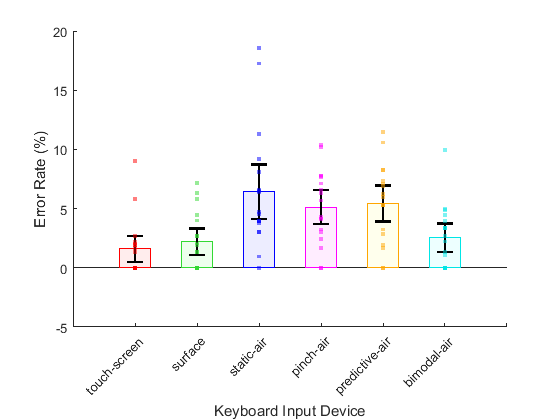
\includegraphics{Figures/fig_MSD_short_mean}
	\caption[Mean Minimum String Distance for Modified-shortest]{Mean Minimum String Distance using the shortest-transcribed modification for each keyboard with error bars showing 95\% confidence intervals.}
	\label{fig_MSD_short_mean}
\end{figure}

The multiple comparisons, seen in Table~\ref{MSD_short_multcompare}, revealed significant differences ($p$-values $<$ 0.05) in Minimum String Distance with the shortest-transcribed modification between the Touch Screen Keyboard and the Leap Static-air, Pinch-air, and Predictive-air keyboards. There were significant differences ($p$-values $<$ 0.05) between the Leap Surface Keyboard and the Leap Static-air and Predictive-air keyboards both. There was also a significant difference ($p$-value $=$ 0.0067) found between the Leap Bimodal-air and the Static-air keyboards.

The error rates seen for the Pinch-air and Touch Screen keyboards for MSD with the shortest-transcribed modification were similar to those found in Vulture for their MWD \cite{ref_vulture}. It is expected that with practice or repeated sessions, these error rates would become even less. The keyboards again follow the same pattern as other measures, providing more evidence of the effects of decoupling on performance and complexity when using 3-dimensions versus a tangible surface. Notably, the Leap Bimodal-air seems to be mostly unaffected by decoupling between the motor space and display space and seems to be only minimally affected by complexity, only having been significantly different from the Touch Screen Keyboard for text-entry rates.

\subsection{Total Error Rate}
Participants reached a mean Total Error Rate of 4.9\% ($SD = 5.5$) for the Touch Screen Keyboard, 9.3\% ($SD = 7.1$) for the Leap Surface Keyboard, 23.6\% ($SD = 12.1$) for the Leap Static-air Keyboard, 14.1\% ($SD = 9.0$) for the Leap Pinch-air Keyboard, 20.1\% ($SD = 11.4$) for the Predictive-air Keyboard, and 6.8\% ($SD = 5.5$) for the Leap Bimodal-air Keyboard. Figure~\ref{fig_totER_mean} shows the mean Total Error Rate for each keyboard interaction style. Using a one-way ANOVA, a significant difference was detected between keyboard means ($F(5, 102) = 12.9381$, $p$-value $<$ 0.0001, $SD_{pooled} = 8.8$), prompting the use of Tukey's HSD with multiple-compare for further analysis.

\begin{figure}[!t]
	\centering
	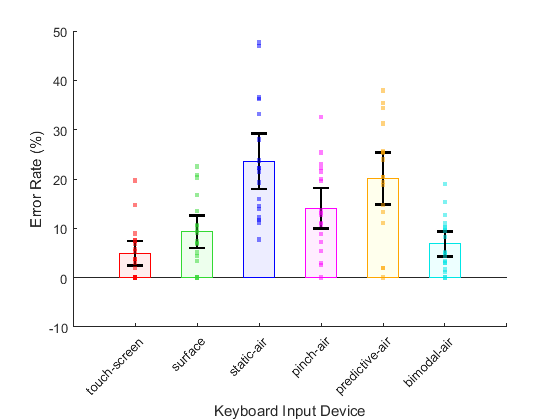
\includegraphics{Figures/fig_totER_mean}
	\caption[Mean Total Error Rates]{Mean Total Error Rates for each keyboard with error bars showing 95\% confidence intervals.}
	\label{fig_totER_mean}
\end{figure}

The multiple comparisons, seen in Table~\ref{totER_multcompare}, revealed significant differences ($p$-values $<$ 0.0001) in Total Error Rate between the Touch Screen Keyboard and the Leap Static-air and Predictive-air keyboards. There were significant differences ($p$-values $<$ 0.01) between the Leap Surface Keyboard and the Static-air and Predictive-air keyboards. There were also significant differences ($p$-values $<$ 0.01) found between the Leap Bimodal-air and the Static-air and Predictive-air keyboards. Finally, there was a significant difference ($p$-value = 0.0191) between the Pinch-air and the Static-air keyboards.

Again, the keyboards follow the same pattern. The Bimodal-air and Leap Surface keyboards perform approximately as well as the Touch Screen Keyboard while the Static-air and Predictive-air keyboards continue to fall short. The Pinch-air keyboard falls somewhere in the middle for Total Error Rate, showing no significant differences with any keyboards.

\subsubsection{Total error rate modified-shortest}
Participants reached a mean Total Error Rate of 4.9\% ($SD = 5.4$) for the Touch Screen Keyboard, 9.2\% ($SD = 7.0$) for the Leap Surface Keyboard, 23.3\% ($SD = 11.8$) for the Leap Static-air Keyboard, 13.5\% ($SD = 8.9$) for the Leap Pinch-air Keyboard, 19.4\% ($SD = 10.7$) for the Predictive-air Keyboard, and 6.7\% ($SD = 5.3$) for the Leap Bimodal-air Keyboard. Figure~\ref{fig_totER_short_mean} shows the mean Total Error Rate with the shortest-transcribed modification for each keyboard interaction style. Using a one-way ANOVA, a significant difference was detected between keyboard means ($F(5, 102) = 13.0717$, $p$-value $<$ 0.0001, $SD_{pooled} = 8.6$), prompting the use of Tukey's HSD with multiple-compare for further analysis.

\begin{figure}[!b]
	\centering
	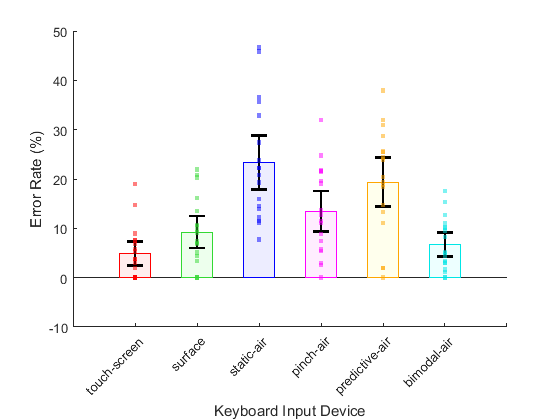
\includegraphics{Figures/fig_totER_short_mean}
	\caption[Mean Total Error Rate for Modified-shortest]{Mean Total Error Rate using the shortest-transcribed modification for each keyboard with error bars showing 95\% confidence intervals.}
	\label{fig_totER_short_mean}
\end{figure}

The multiple comparisons, seen in Table~\ref{totER_short_multcompare}, revealed significant differences ($p$-values $<$ 0.05) in Total Error Rate with the shortest-transcribed modification between the Touch Screen Keyboard and the Leap Static-air, Pinch-air, and Predictive-air keyboards. There were significant differences ($p$-values $<$ 0.01) between the Leap Surface Keyboard and the Leap Static-air and Predictive-air keyboards. There were also significant differences found between the Leap Bimodal-air and the Static-air and Predictive-air keyboards with a $p$-value $<$ 0.001. Finally, there was a significant difference ($p$-value = 0.0101) between the Pinch-air and Static-air keyboards.

Surprisingly, unlike KSPC and MWD, the Total Error Rate did not follow suit by showing large decreases in error rate with the shortest-transcribed modification. However, these observations continue to support the findings between the text-entry rates with and without modification, which were also relatively unaffected by the shortest-transcribed modification. This further implied that errors made by participants were more likely corrected throughout gesturing words rather than after having completed the word-gesture. This was a major downside of lacking word-recognition because gestures were interrupted and corrected rather than being completed with errors, as is natural to traditional word-gesture keyboards.

\section{Correctness}
\subsection{Fr\'echet Distance} \label{results_frechet}
Participants reached a mean Fr\'echet Distance of 231.2 pixels ($SD = 26.7$) for the Touch Screen Keyboard, 242.8 pixels ($SD = 30.4$) for the Leap Surface Keyboard, 364.3 pixels ($SD = 86.5$) for the Leap Static-air Keyboard, 501.2 pixels ($SD = 42.8$) for the Leap Pinch-air Keyboard, 350.6 pixels ($SD = 86.8$) for the Predictive-air Keyboard, and 396.5 pixels ($SD = 102.1$) for the Leap Bimodal-air Keyboard. Figure~\ref{fig_frechet_mean} shows the mean Fr\'echet Distance for each keyboard interaction style. Using a one-way ANOVA, a significant difference was detected between keyboard means ($F(5, 102) = 37.9416$, $p$-value $<$ 0.0001, $SD_{pooled} = 69.4$), prompting the use of Tukey's HSD with multiple-compare for further analysis.

\begin{figure}[!t]
	\centering
	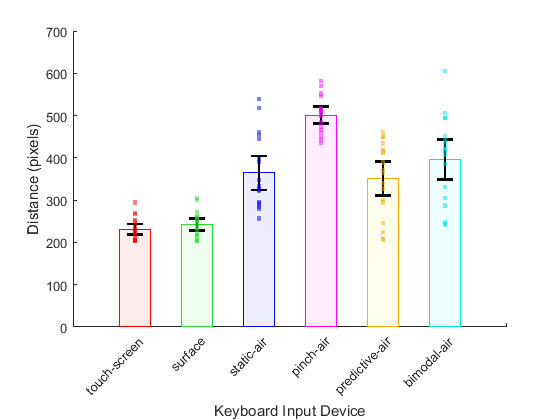
\includegraphics{Figures/fig_frechet_mean}
	\caption[Mean Fr\'echet Distance]{Mean Fr\'echet Distance for each keyboard with error bars showing 95\% confidence intervals.}
	\label{fig_frechet_mean}
\end{figure}

The multiple comparisons, seen in Table~\ref{frechet_multcompare}, revealed significant differences ($p$-values $<$ 0.0001) in Fr\'echet Distance between the Touch Screen Keyboard and all of the mid-air keyboards. There were significant differences ($p$-values $<$ 0.001) between the Leap Surface Keyboard and all of the mid-air keyboards. There were also significant differences ($p$-values $<$ 0.001) found between the Leap Pinch-air and all of the other mid-air keyboards.

The Fr\'echet Distance was the only place where the trends were broken and the Bimodal-air keyboard performed significantly worse than the Touch Screen and Leap Surface keyboards. The Pinch-air Keyboard also performed significantly worse than all other keyboards. These results were assumed to be caused by a combination of the word-gesture velocity seen in Section~\ref{results_velocity_gesture} and the effects of either increased decoupling or complexity from working with the 3rd-dimension. Appendix~\ref{user_generated_paths} emphasizes these assumptions by illustrating the participant-generated word-gesture paths for all word sets and their corresponding keyboards.

The Leap Bimodal-air seemed to suffer in correctness due to its very high word-gesture velocities, whereas the Static-air and Predictive-air benefit in correctness due to their very slow word-gesture velocities. Participants used explicitly slower, more precise gestures to compensate for these keyboards' increased decoupling. The Leap Surface and Touch Screen keyboards were relatively unaffected in correctness by their high word-gesturing velocities due to their decreased decoupling of the word-gesture motor space from the displayed screen.

The Pinch-air Keyboard suffered from the combination of high word-gesture velocities and effects of increased decoupling. However, the Pinch-air Keyboard also seemed to be heavily affected by the deviation in its tracking method, which increased the overall distance traveled for each word-gesture, as seen in Section~\ref{results_distance}. All other mid-air keyboards tracked participants' pointer fingers, whereas the Pinch-air keyboard tracked participants' palms. Palms were tracked instead because participants' fingers moved drastically when creating a pinching gesture. This difference in tracking combined with high word-gesture velocities were the assumed factors for this decrease in performance.

\subsubsection{Fr\'echet distance modified-shortest}
Participants reached a mean Fr\'echet Distance of 221.0 pixels ($SD = 18.0$) for the Touch Screen Keyboard, 231.0 pixels ($SD = 22.7$) for the Leap Surface Keyboard, 306.4 pixels ($SD = 53.2$) for the Leap Static-air Keyboard, 459.2 pixels ($SD = 20.1$) for the Leap Pinch-air Keyboard, 281.6 pixels ($SD = 49.9$) for the Predictive-air Keyboard, and 368.4 pixels ($SD = 82.4$) for the Leap Bimodal-air Keyboard. Figure~\ref{fig_frechet_short_mean} shows the mean Fr\'echet Distance with the shortest-transcribed modification for each keyboard interaction style. Using a one-way ANOVA, a significant difference was detected between keyboard means ($F(5, 102) = 65.7440$, $p$-value $<$ 0.0001, $SD_{pooled} = 47.2$), prompting the use of Tukey's HSD with multiple-compare for further analysis.

\begin{figure}[!t]
	\centering
	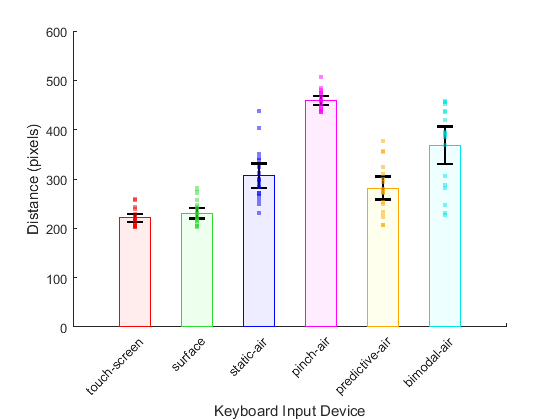
\includegraphics{Figures/fig_frechet_short_mean}
	\caption[Mean Fr\'echet Distance for Modified-shortest]{Mean Fr\'echet Distance using the shortest-transcribed modification for each keyboard with error bars showing 95\% confidence intervals.}
	\label{fig_frechet_short_mean}
\end{figure}

The multiple comparisons, seen in Table~\ref{frechet_short_multcompare}, revealed significant differences ($p$-values $<$ 0.01) in Fr\'echet Distance with the shortest-transcribed modification between the Touch Screen Keyboard and all of the mid-air keyboards. There were significant differences ($p$-values $<$ 0.05) between the Leap Surface Keyboard and all of the mid-air keyboards. There were also significant differences ($p$-values $<$ 0.01) found between the Leap Bimodal-air Keyboard and the other mid-air keyboards. Finally, there were significant differences ($p$-values $<$ 0.0001) found between the Leap Pinch-air Keyboard and the Static-air and Predictive-air keyboards.

The increased correctness for all keyboards, especially the mid-air keyboards, when using the shortest-transcribed modification implies that many errors were being produced when exiting the interaction plane. This was especially evident for the Static-air, Pinch-air, and Predictive-air keyboards, which all saw the largest improvements to correctness. For the Static-air and Predictive-air keyboards, these errors were caused by the addition of the 3rd-dimension and participants having trouble entering and exiting the interaction plane accurately. The Pinch-air Keyboard saw a combination of high word-gesture velocity and a different method of tracking that was assumed to produce these kinds of errors.

\subsubsection{Fr\'echet distance modified-backspace}
Participants reached a mean Fr\'echet Distance of 212.3 pixels ($SD = 9.3$) for the Touch Screen Keyboard, 223.5 pixels ($SD = 18.5$) for the Leap Surface Keyboard, 258.9 pixels ($SD = 33.5$) for the Leap Static-air Keyboard, 444.7 pixels ($SD = 8.0$) for the Leap Pinch-air Keyboard, 237.7 pixels ($SD = 24.8$) for the Predictive-air Keyboard, and 356.8 pixels ($SD = 85.0$) for the Leap Bimodal-air Keyboard. Figure~\ref{fig_frechet_back_mean} shows the mean Fr\'echet Distance with the backspace-transcribed modification for each keyboard interaction style. Using a one-way ANOVA, a significant difference was detected between keyboard means ($F(5, 102) = 97.1196$, $p$-value $<$ 0.0001, $SD_{pooled} = 39.7$), prompting the use of Tukey's HSD with multiple-compare for further analysis.

\begin{figure}[!t]
	\centering
	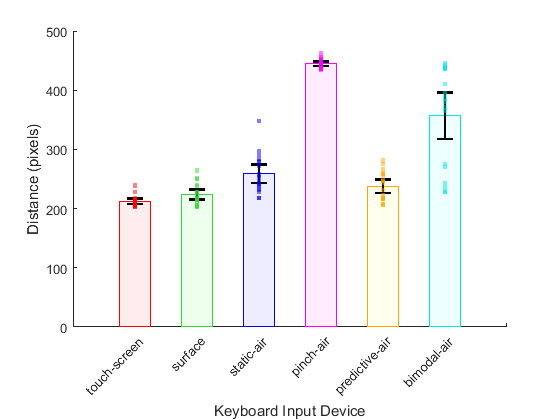
\includegraphics{Figures/fig_frechet_back_mean}
	\caption[Mean Fr\'echet Distance for Modified-backspace]{Mean Fr\'echet Distance using the backspace-transcribed modification for each keyboard with error bars showing 95\% confidence intervals.}
	\label{fig_frechet_back_mean}
\end{figure}

The multiple comparisons, seen in Table~\ref{frechet_back_multcompare}, revealed significant differences ($p$-values $<$ 0.01) in Fr\'echet Distance with the backspace-transcribed modification between the Touch Screen Keyboard and the Leap Static-air, Pinch-air, and Bimodal-air keyboards. There were significant differences ($p$-values $<$ 0.0001) between the Leap Surface Keyboard and the Leap Pinch-air and Bimodal-air keyboards. There were also significant differences ($p$-values $<$ 0.0001) found between the Leap Bimodal-air and all other mid-air keyboards. Finally, there were significant differences ($p$-values $<$ 0.0001) between the Leap Pinch-air Keyboard and the Static-air and Predictive-air keyboards.

If the backspace key was included in the path considered to be correct for Fr\'echet Distance, since participants were required to correct words, a boost in correctness was observed. The Bimodal-air and Pinch-air keyboards still suffered from the previously mentioned problems in Section~\ref{results_frechet}. The Static-air and Predictive-air, however, saw huge improvements in correctness because of the low word-gesture velocities and high error rates. The Predictive-air Keyboard, in this case, was not significantly different from the Touch Screen and Leap Surface keyboards, implying that participants were relatively attentive to correcting errors for it.

\section{Distance Measures}
\subsection{Word-gesture Distance} \label{results_distance}
Participants reached a mean Word-gesture Distance of 1087.5 pixels ($SD = 85.9$) for the Touch Screen Keyboard, 1423.9 pixels ($SD = 246.0$) for the Leap Surface Keyboard, 1590.9 pixels ($SD = 508.2$) for the Leap Static-air Keyboard, 2165.3 pixels ($SD = 540.5$) for the Leap Pinch-air Keyboard, 1634.7 pixels ($SD = 481.4$) for the Predictive-air Keyboard, and 1627.7 pixels ($SD = 321.3$) for the Leap Bimodal-air Keyboard. Figure~\ref{fig_distance_mean} shows the mean Word-gesture Distance for each keyboard interaction style. Using a one-way ANOVA, a significant difference was detected between keyboard means ($F(5, 102) = 13.9225$, $p$-value $<$ 0.0001, $SD_{pooled} = 398.6$), prompting the use of Tukey's HSD with multiple-compare for further analysis.

\begin{figure}[!t]
	\centering
	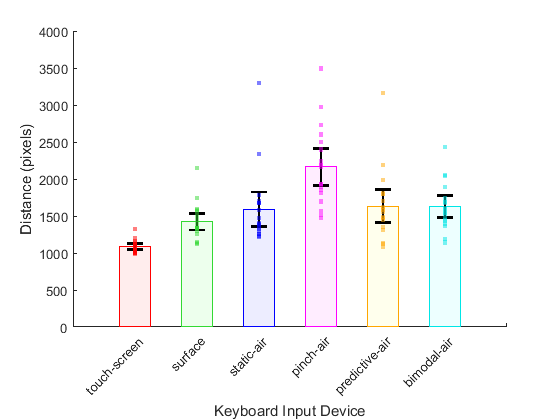
\includegraphics{Figures/fig_distance_mean}
	\caption[Mean Word-gesture Distance]{Mean Word-gesture Distance for each keyboard with error bars showing 95\% confidence intervals.}
	\label{fig_distance_mean}
\end{figure}

The multiple comparisons, seen in Table~\ref{distance_multcompare}, revealed significant differences ($p$-values $<$ 0.01) in Word-gesture Distance between the Touch Screen Keyboard and all of the mid-air keyboards. There were also significant differences ($p$-values $<$ 0.01) between the Leap Pinch-air and all other Leap Motion-based keyboards.

As expected, all mid-air keyboards required longer word-gesture distances than the Touch Screen Keyboard due to the effect of decoupling between the word-gesture motor space and the keyboard display. It was surprising, however, that the Leap Surface Keyboard required significantly more word-gesture distance than the Touch Screen Keyboard. This could be because of the requirement to use a stylus rather than the participants' bare hands.

The Pinch-air keyboard required a significantly longer word-gesture distance than all other keyboards. This was assumed to be caused by the different tracking method as previously mentioned. Tracking the palm required broader, less controlled movements than tracking fingers or a stylus.

\subsubsection{Word-gesture distance modified-shortest}
Participants reached a mean Word-gesture Distance of 1081.3 ($SD = 84.6$) for the Touch Screen Keyboard, 1396.5 ($SD = 226.5$) for the Leap Surface Keyboard, 1524.8 ($SD = 412.5$) for the Leap Static-air Keyboard, 1981.4 ($SD = 470.6$) for the Leap Pinch-air Keyboard, 1536.7 ($SD = 346.1$) for the Predictive-air Keyboard, and 1566.5 ($SD = 253.6$) for the Leap Bimodal-air Keyboard. Figure~\ref{fig_distance_short_mean} shows the mean Word-gesture Distance with the shortest-transcribed modification for each keyboard interaction style. Using a one-way ANOVA, a significant difference was detected between keyboard means ($F(5, 102) = 14.403$, $p$-value $<$ 0.0001, $SD_{pooled} = 325.1$), prompting the use of Tukey's HSD with multiple-compare for further analysis.

\begin{figure}[!t]
	\centering
	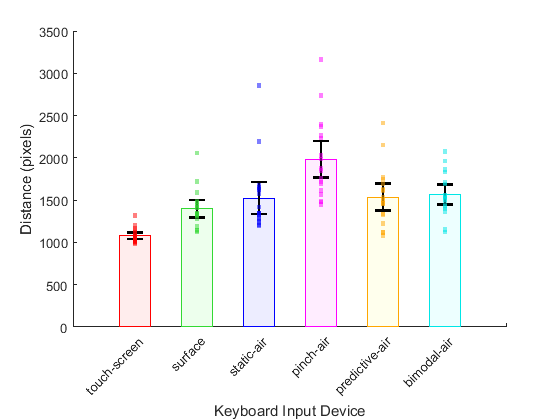
\includegraphics{Figures/fig_distance_short_mean}
	\caption[Mean Word-gesture Distance for Modified-shortest]{Mean Word-gesture Distance using the shortest-transcribed modification for each keyboard with error bars showing 95\% confidence intervals.}
	\label{fig_distance_short_mean}
\end{figure}

The multiple comparisons, seen in Table~\ref{distance_short_multcompare}, revealed significant differences ($p$-values $<$ 0.05) in Word-gesture Distance with the shortest-transcribed modification between the Touch Screen Keyboard and all other keyboards. There were significant differences ($p$-values $<$ 0.01) between the Leap Surface and Pinch-air keyboards and all other Leap Motion-based keyboards.

Again, the small difference between the word-gesture distance and the word-gesture distance using the shortest-transcribed modification implied that most errors were corrected by participants while in the middle of typing words.

\subsection{Word-gesture Velocity} \label{results_velocity_gesture}
Participants reached a mean Word-gesture Velocity of 673.3 $pixels/s$ ($SD = 126.4$) for the Touch Screen Keyboard, 641.1 $pixels/s$ ($SD = 165.5$) for the Leap Surface Keyboard, 380.9 $pixels/s$ ($SD = 78.2$) for the Leap Static-air Keyboard, 643.8 $pixels/s$ ($SD = 204.7$) for the Leap Pinch-air Keyboard, 405.6 $pixels/s$ ($SD = 87.6$) for the Predictive-air Keyboard, and 777.6 $pixels/s$ ($SD = 240.9$) for the Leap Bimodal-air Keyboard. Figure~\ref{fig_velocity_gesture_mean} shows the mean Word-gesture Velocity for each keyboard interaction style. Using a one-way ANOVA, a significant difference was detected between keyboard means ($F(5, 102) = 17.233$, $p$-value $<$ 0.0001, $SD_{pooled} = 161.8$), prompting the use of Tukey's HSD with multiple-compare for further analysis.

\begin{figure}[h]
	\centering
	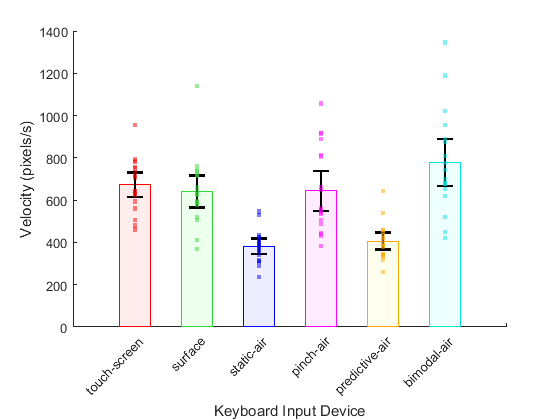
\includegraphics{Figures/fig_velocity_gesture_mean}
	\caption[Mean Word-gesture Velocity]{Mean Word-gesture Velocity for each keyboard with error bars showing 95\% confidence intervals.}
	\label{fig_velocity_gesture_mean}
\end{figure}

The multiple comparisons, seen in Table~\ref{velocity_gesture_multcompare}, revealed significant differences ($p$-values $<$ 0.0001) in Word-gesture Velocity between the Touch Screen Keyboard and the Leap Static-air and Predictive-air keyboards. There were significant differences ($p$-values $<$ 0.001) between the Leap Surface Keyboard and the Static-air and Predictive-air keyboards. There were also significant differences ($p$-values $<$ 0.0001) found between the Leap Bimodal-air and the Static-air and Predictive-air keyboards. Finally, there were significant differences ($p$-values $<$ 0.001) found between the Leap Pinch-air and the Static-air and Predictive Air keyboards.

The Static-air and Predictive-air keyboards were significantly slower than all of the other keyboards for word-gesture velocity. This was expected due to the enhanced precision required when working with a 3rd-dimension in mid-air. It is interesting that these two keyboards also had the highest error rates across all error measures, implying a very high degree of difficulty, even with slower, more precise movements.

\subsection{Hand Velocity}
Participants reached a mean Hand Velocity of 35.7 $cm/s$ ($SD = 6.7$) for the Touch Screen Keyboard, 15.0 $cm/s$ ($SD = 3.9$) for the Leap Surface Keyboard, 6.9 $cm/s$ ($SD = 1.4$) for the Leap Static-air Keyboard, 10.5 $cm/s$ ($SD = 3.2$) for the Leap Pinch-air Keyboard, 7.6 $cm/s$ ($SD = 1.7$) for the Predictive-air Keyboard, and 15.2 $cm/s$ ($SD = 5.1$) for the Leap Bimodal-air Keyboard. Figure~\ref{fig_velocity_hand_mean} shows the mean Hand Velocity for each keyboard interaction style. Using a one-way ANOVA, a significant difference was detected between keyboard means ($F(5, 102) = 121.9826$, $p$-value $<$ 0.0001, $SD_{pooled} = 4.1$), prompting the use of Tukey's HSD with multiple-compare for further analysis.

\begin{figure}[!t]
	\centering
	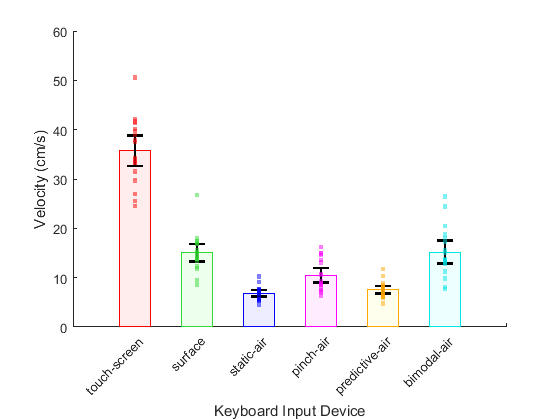
\includegraphics{Figures/fig_velocity_hand_mean}
	\caption[Mean Hand Velocity]{Mean Hand Velocity for each keyboard with error bars showing 95\% confidence intervals.}
	\label{fig_velocity_hand_mean}
\end{figure}

The multiple comparisons, seen in Table~\ref{velocity_hand_multcompare}, revealed significant differences ($p$-values $<$ 0.0001) in Hand Velocity between the Touch Screen Keyboard and all other keyboards. There were significant differences ($p$-values $<$ 0.05) between the Leap Surface Keyboard and the Static-air, Pinch-air, and Predictive-air keyboards. There were also significant differences ($p$-values $<$ 0.05) found between the Leap Bimodal-air and all other mid-air keyboards.

The hand velocities were all similar to the word-gesture velocities in Section~\ref{results_velocity_gesture}, except for the Touch Screen Keyboard. This result was simply caused by the physical size difference between the interaction planes and the size of the Touch Screen, as mentioned in Chapter~\ref{keyboard_design}.

\section{Time-based Measures}

\subsection{Word-gesture Duration}
Participants reached a mean Word-gesture Duration of 1.65 $s$ ($SD = 0.46$) for the Touch Screen Keyboard, 2.03 $s$ ($SD = 1.17$) for the Leap Surface Keyboard, 4.01 $s$ ($SD = 1.17$) for the Leap Static-air Keyboard, 3.36 $s$ ($SD = 0.76$) for the Leap Pinch-air Keyboard, 3.87 $s$ ($SD = 1.18$) for the Predictive-air Keyboard, and 2.18 $s$ ($SD = 0.36$) for the Leap Bimodal-air Keyboard. Figure~\ref{fig_time_mean} shows the mean Word-gesture Duration for each keyboard interaction style. Using a one-way ANOVA, a significant difference was detected between keyboard means ($F(5, 102) = 28.1205$, $p$-value $<$ 0.0001, $SD_{pooled} = 0.81$), prompting the use of Tukey's HSD with multiple-compare for further analysis.

\begin{figure}[!b]
	\centering
	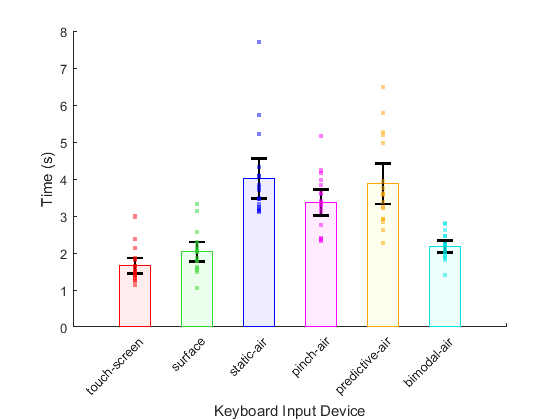
\includegraphics{Figures/fig_time_mean}
	\caption[Mean Word-gesture Duration]{Mean Word-gesture Duration for each keyboard with error bars showing 95\% confidence intervals.}
	\label{fig_time_mean}
\end{figure}

The multiple comparisons, seen in Table~\ref{time_multcompare}, revealed significant differences ($p$-values $<$ 0.0001) in Word-gesture Duration between the Touch Screen Keyboard and the Leap Static-air, Pinch-air, and Predictive-air keyboards. There were significant differences ($p$-values $<$ 0.001) between the Leap Surface Keyboard and the Static-air, Pinch-air, and Predictive-air keyboards. There were also significant differences ($p$-values $<$ 0.001) found between the Leap Bimodal-air and all of the other mid-air keyboards.

As expected, the Static-air, Pinch-air, and Predictive-air keyboards had significantly longer word-gesture durations than the other keyboards. For the Static-air and Predictive-air, lower velocities and higher decoupling meant that word-gestures take longer to perform, whereas for the Pinch-air Keyboard, the longer distances traveled influenced the longer durations. The Bimodal-air keyboard performed as well as the Touch Screen and Leap Surface keyboards, as expected from its prior trends. 

\subsubsection{Word-gesture duration modified-shortest}
Participants reached a mean Word-gesture Duration of 1.60 $s$ ($SD = 0.40$) for the Touch Screen Keyboard, 2.00 $s$ ($SD = 0.55$) for the Leap Surface Keyboard, 3.75 $s$ ($SD = 0.93$) for the Leap Static-air Keyboard, 3.17 $s$ ($SD = 0.73$) for the Leap Pinch-air Keyboard, 3.56 $s$ ($SD = 0.86$) for the Predictive-air Keyboard, and 2.16 $s$ ($SD = 0.36$) for the Leap Bimodal-air Keyboard. Figure~\ref{fig_time_short_mean} shows the mean Word-gesture Duration with the shortest-transcribed modification for each keyboard interaction style. Using a one-way ANOVA, a significant difference was detected between keyboard means ($F(5, 102) = 32.0355$, $p$-value $<$ 0.0001, $SD_{pooled} = 0.67$), prompting the use of Tukey's HSD with multiple-compare for further analysis.

\begin{figure}[!t]
	\centering
	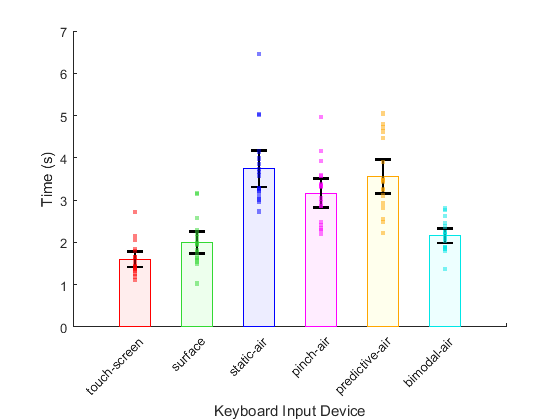
\includegraphics{Figures/fig_time_short_mean}
	\caption[Mean Word-gesture Duration for Modified-shortest]{Mean Word-gesture Dur using the shortest-transcribed modification for each keyboard with error bars showing 95\% confidence intervals.}
	\label{fig_time_short_mean}
\end{figure}

The multiple comparisons, seen in Table~\ref{time_short_multcompare}, revealed significant differences ($p$-values $<$ 0.0001) in Word-gesture Duration with the shortest-transcribed modification between the Touch Screen Keyboard and the Leap Static-air, Pinch-air, and Predictive-air keyboards. There were significant differences ($p$-values $<$ 0.0001) between the Leap Surface Keyboard and the Leap Static-air, Pinch-air, and Predictive-air keyboards. There were also significant differences ($p$-values $<$ 0.001) found between the Leap Bimodal-air and all of the other mid-air keyboards.

As seen before, the shortest-transcribed modification for word-gesture duration had little effect on the total length of word-gesture durations. This again supported the idea that participants mostly corrected errors as they were being made during transcription.

\subsection{Reaction Time to Errors}
Participants reached a mean Reaction Time to Errors of 0.22 $s$ ($SD = 0.23$) for the Touch Screen Keyboard, 0.40 $s$ ($SD = 0.29$) for the Leap Surface Keyboard, 1.02 $s$ ($SD = 0.43$) for the Leap Static-air Keyboard, 0.59 $s$ ($SD = 0.30$) for the Leap Pinch-air Keyboard, 0.78 $s$ ($SD = 0.40$) for the Predictive-air Keyboard, and 0.29 $s$ ($SD = 0.24$) for the Leap Bimodal-air Keyboard. Figure~\ref{fig_reaction_errors_mean} shows the mean Reaction Time to Errors for each keyboard interaction style. Using a one-way ANOVA, a significant difference was detected between keyboard means ($F(5, 102) = 16.3385$, $p$-value $<$ 0.0001, $SD_{pooled} = 0.32$), prompting the use of Tukey's HSD with multiple-compare for further analysis.

\begin{figure}[!t]
	\centering
	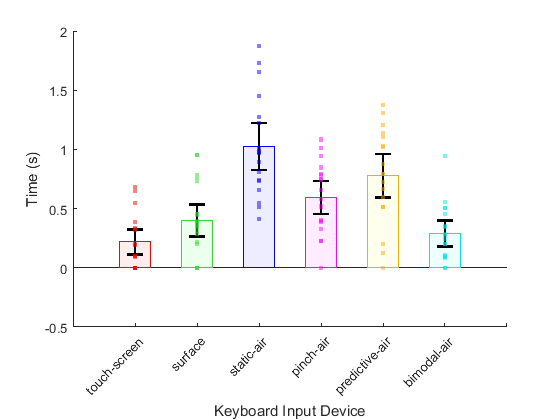
\includegraphics{Figures/fig_reaction_errors_mean}
	\caption[Mean Reaction Time to Errors]{Mean Reaction Time to Errors for each keyboard with error bars showing 95\% confidence intervals.}
	\label{fig_reaction_errors_mean}
\end{figure}

The multiple comparisons, seen in Table~\ref{reaction_errors_multcompare}, revealed significant differences ($p$-values $<$ 0.01) in Reaction Time to Errors between the Touch Screen Keyboard and the Leap Static-air, Pinch-air, and Predictive-air keyboards. There were significant differences ($p$-values $<$ 0.01) between the Leap Surface Keyboard and the Static-air and Predictive-air keyboards. There were also significant differences ($p$-values $<$ 0.001) found between the Leap Bimodal-air and the Static-air and Predictive-air keyboards. Finally, there was a significant difference ($p$-value $=$ 0.0017) found between the Pinch-air and Static-air keyboards.

As expected, keyboards involving the 3rd-dimension had significantly slower response times to errors than keyboards that did not. This implied that these keyboards required a higher degree of focus due to increased decoupling between the motor space and display.

\subsection{Reaction Time to Simulate Touch}
Participants reached a mean Reaction Time to Simulate Touch of 1.24 $s$ ($SD = 0.21$) for the Touch Screen Keyboard, 1.22 $s$ ($SD = 0.40$) for the Leap Surface Keyboard, 2.60 $s$ ($SD = 0.82$) for the Leap Static-air Keyboard, 1.71 $s$ ($SD = 0.37$) for the Leap Pinch-air Keyboard, 2.23 $s$ ($SD = 0.83$) for the Predictive-air Keyboard, and 1.41 $s$ ($SD = 0.23$) for the Leap Bimodal-air Keyboard. Figure~\ref{fig_reaction_touch_mean} shows the mean Reaction Time to Simulate Touch for each keyboard interaction style. Using a one-way ANOVA, a significant difference was detected between keyboard means ($F(5, 102) = 19.6476$, $p$-value $<$ 0.0001, $SD_{pooled} = 0.54$), prompting the use of Tukey's HSD with multiple-compare for further analysis.

\begin{figure}[!t]
	\centering
	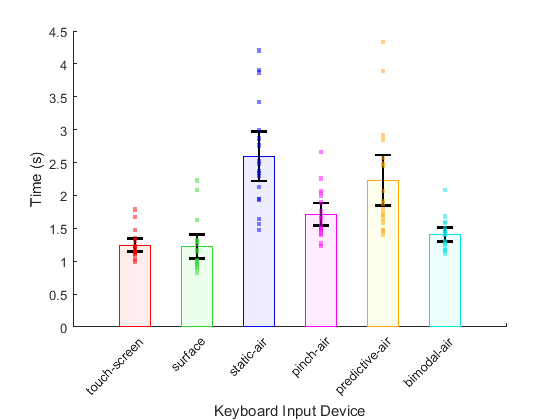
\includegraphics{Figures/fig_reaction_touch_mean}
	\caption[Mean Reaction Time to Simulate Touch]{Mean Reaction Time to Simulate Touch for each keyboard with error bars showing 95\% confidence intervals.}
	\label{fig_reaction_touch_mean}
\end{figure}

The multiple comparisons, seen in Table~\ref{reaction_touch_multcompare}, revealed significant differences ($p$-values $<$ 0.0001) in Reaction Time to Simulate Touch between the Touch Screen Keyboard and the Leap Static-air and Predictive-air keyboards. There were significant differences ($p$-values $<$ 0.0001) between the Leap Surface Keyboard and the Static-air and Predictive-air keyboards. There were also significant differences ($p$-values $<$ 0.001) found between the Leap Bimodal-air and the Static-air and Predictive-air keyboards. Finally, a significant difference ($p$-value = 0.0001) was detected between the Pinch-air and Static-air keyboards.

Again, the reaction time to simulate a touch was significantly slower for the Static-air and Predictive-air keyboards due to the introduction of the 3rd-dimension and increased decoupling between the word-gesture motor space and the display.

\subsection{Reaction Time for First Correct Letter}
Participants reached a mean Reaction Time for First Correct Letter of 1.44 $s$ ($SD = 0.33$) for the Touch Screen Keyboard, 1.92 $s$ ($SD = 0.70$) for the Leap Surface Keyboard, 3.68 $s$ ($SD = 1.52$) for the Leap Static-air Keyboard, 2.34 $s$ ($SD = 0.68$) for the Leap Pinch-air Keyboard, 3.40 $s$ ($SD = 1.40$) for the Predictive-air Keyboard, and 1.49 $s$ ($SD = 0.31$) for the Leap Bimodal-air Keyboard. Figure~\ref{fig_reaction_pressed_mean} shows the mean Reaction Time for First Correct Letter for each keyboard interaction style. Using a one-way ANOVA, a significant difference was detected between keyboard means ($F(5, 102) = 18.3416$, $p$-value $<$ 0.0001, $SD_{pooled} = 0.95$), prompting the use of Tukey's HSD with multiple-compare for further analysis.

\begin{figure}[!t]
	\centering
	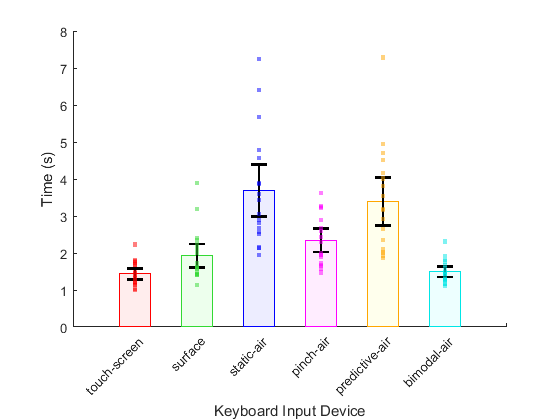
\includegraphics{Figures/fig_reaction_pressed_mean}
	\caption[Mean Reaction Time for First Correct Letter]{Mean Reaction Time for First Correct Letter for each keyboard with error bars showing 95\% confidence intervals.}
	\label{fig_reaction_pressed_mean}
\end{figure}

The multiple comparisons, seen in Table~\ref{reaction_pressed_multcompare}, revealed significant differences ($p$-values $<$ 0.0001) in Reaction Time for First Correct Letter between the Touch Screen Keyboard and the Leap Static-air and Predictive-air keyboards. There were significant differences ($p$-values $<$ 0.001) between the Leap Surface Keyboard and the Static-air and Predictive-air keyboards. There were also significant differences ($p$-values $<$ 0.0001) found between the Leap Bimodal-air and the Static-air and Predictive-air keyboards. Finally, there were significant differences ($p$-values $<$ 0.05) found between the Leap Pinch-air and the Static-air and Predictive-air keyboards.

The Leap Bimodal-air Keyboard performed at almost exactly the same rate as the Touch Screen Keyboard for entering the first correct character of each word. Although not a significant difference, it should also be noted that the Leap Surface Keyboard performed slightly slower than both the Bimodal-air and Touch Screen keyboards because participants had a tendency to look down at the printed keyboard. If participants had looked at the on-screen keyboard instead, there would have been a major increase in decoupling that would have further slowed the use of the Leap Surface Keyboard.

Again, the reaction time to simulate a touch was significantly slower for the Static-air and Predictive-air keyboards due to the introduction of the 3rd-dimension and increased decoupling between the word-gesture motor space and the display.

\section{Additional Quantitative Measures}

\subsection{Number of Touches Simulated}
Participants reached a mean Number of Touches Simulated of 1.58 simulations ($SD = 0.79$) for the Touch Screen Keyboard, 1.62 simulations ($SD = 0.55$) for the Leap Surface Keyboard, 3.77 simulations ($SD = 2.21$) for the Leap Static-air Keyboard, 2.42 simulations ($SD = 1.05$) for the Leap Pinch-air Keyboard, 3.33 simulations ($SD = 1.62$) for the Predictive-air Keyboard, and 1.67 simulations ($SD = 0.53$) for the Leap Bimodal-air Keyboard. Figure~\ref{fig_num_touches_mean} shows the mean Number of Touches Simulated for each keyboard interaction style. Using a one-way ANOVA, a significant difference was detected between keyboard means ($F(5, 102) = 10.0290$, $p$-value $<$ 0.0001, $SD_{pooled} = 1.28$), prompting the use of Tukey's HSD with multiple-compare for further analysis.

\begin{figure}[!t]
	\centering
	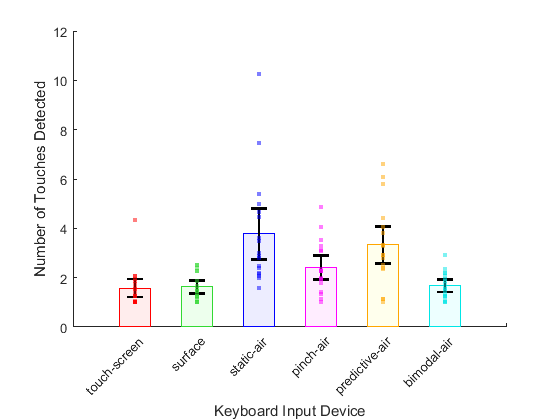
\includegraphics{Figures/fig_num_touches_mean}
	\caption[Mean Number of Touches Simulated]{Mean Number of Touches Simulated for each keyboard with error bars showing 95\% confidence intervals.}
	\label{fig_num_touches_mean}
\end{figure}

The multiple comparisons, seen in Table~\ref{num_touches_multcompare}, revealed significant differences ($p$-values $<$ 0.01) in Number of Touches Simulated between the Touch Screen Keyboard and the Leap Static-air and Predictive-air keyboards. There were significant differences ($p$-values $<$ 0.01) between the Leap Surface Keyboard and the Static-air and Predictive-air keyboards. There were also significant differences ($p$-values $<$ 0.01) found between the Leap Bimodal-air and the Static-air and Predictive-air keyboards. Finally, there was a significant difference ($p$-value = 0.0245) between the Pinch-air keyboard and the Static-air keyboard.

Again, the same trends as before were seen. The Leap Surface and Bimodal-air keyboards performed on par with the Touch Screen Keyboard, the Static-air and Predictive-air keyboards saw significantly more simulated touches, and the Pinch-air keyboard was somewhere in the middle. It was observed that the Static-air keyboard suffered from a ``skimming'' issue. The ``skimming'' issue occurred when participants would only reach far enough to barely simulate a touch on the interaction plane, and then when they would move their hand from one side of the keyboard to the other, the natural arcing motion of the participants' hands would cause them to pull away from the interaction plane as they moved. This issue was assumed to also be a culprit for some of the increased error rates. Figure~\ref{arcing_motion} and Figure~\ref{skimming_problem} both show how the skimming issue worked in detail. % TODO: possibly move skimming problem figure from conclusion to here

\subsection{Number of Practice Words}
Participants reached a mean Number of Practice Words of 5.4 words ($SD = 4.3$) for the Touch Screen Keyboard, 7.7 words ($SD = 3.9$) for the Leap Surface Keyboard, 9.0 words ($SD = 6.7$) for the Leap Static-air Keyboard, 8.1 words ($SD = 5.3$) for the Leap Pinch-air Keyboard, 8.9 words ($SD = 6.8$) for the Predictive-air Keyboard, and 10.2 words ($SD = 3.9$) for the Leap Bimodal-air Keyboard. Figure~\ref{fig_num_practice_mean} shows the mean Number of Practice Words for each keyboard interaction style. Using a one-way ANOVA, no significant differences were detected between keyboard means ($F(5, 102) = 1.6828$, $p$-value = 0.1454, $SD_{pooled} = 5.3$), therefore no additional analysis was made. Typically, as observed by the researcher, there were two categories of participants when it came to performing practice words. The first category contained participants who would perform a full set of 15 words for each keyboard. Rarely, these participants felt the need to perform more than one practice set's worth of words. The second category contained participants who progressively performed less practice words for each consecutive keyboard; this is a primary example of why a Replicated Latin Squares design for counterbalancing was used.

\begin{figure}[!t]
	\centering
	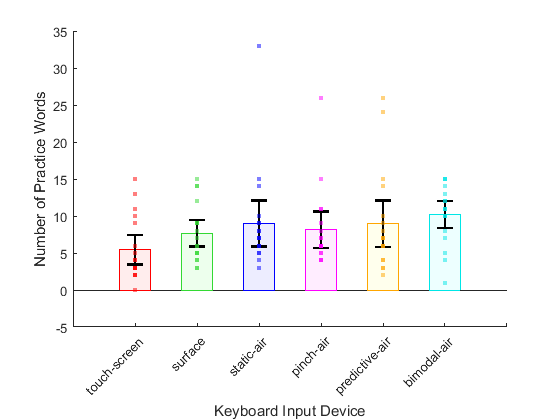
\includegraphics{Figures/fig_num_practice_mean}
	\caption[Mean Number of Practice Words]{Mean Number of Practice Words for each keyboard with error bars showing 95\% confidence intervals.}
	\label{fig_num_practice_mean}
\end{figure}

\section{Qualitative Measures}
\subsection{Level of Discomfort}
%means = -1.7222   -1.5556   -0.2778   -0.7778   -0.3889   -1.2778
%stds = 0.7519    0.6157    1.0741    0.9428    1.3346    0.7519
Keyboards reached a median Level of Discomfort of ``Strongly Disagree'' for the Touch Screen Keyboard, ``Strongly Disagree'' for the Leap Surface Keyboard, ``Neutral'' for the Leap Static-air Keyboard, ``Disagree'' for the Leap Pinch-air Keyboard, between ``Disagree'' and ``Neutral'' for the Predictive-air Keyboard, and ``Disagree'' for the Leap Bimodal-air Keyboard. Figure~\ref{fig_discomfort_boxplot} shows the median Level of Discomfort for each keyboard interaction style rated by the participants. Using a one-way ANOVA, a significant difference was detected between keyboard means for Level of Discomfort ($F(5, 102) = 7.5000$, $p$-value $<$ 0.0001, $SD_{pooled} = 0.94$), prompting the use of Tukey's HSD with multiple-compare for further analysis.

\begin{figure}[!t]
	\centering
	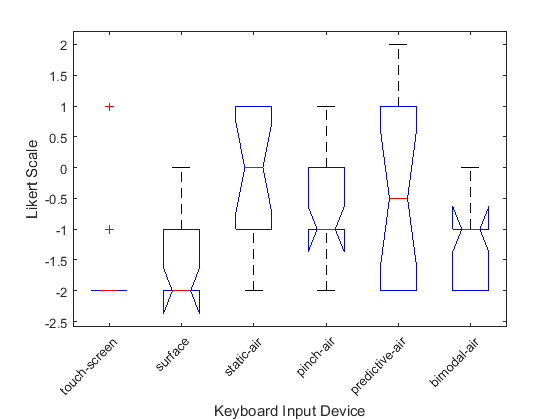
\includegraphics{Figures/fig_discomfort_boxplot}
	\caption[Level of Discomfort Boxplot]{Median Level of Discomfort for each keyboard showing the 25th and 75th percentiles.}
	\label{fig_discomfort_boxplot}
\end{figure}

The multiple comparisons, seen in Table~\ref{discomfort_multcompare}, revealed significant differences ($p$-values $<$ 0.05) in Level of Discomfort between the Touch Screen Keyboard and the Leap Static-air, Pinch-air, and Predictive-air keyboards. There were significant differences ($p$-values $<$ 0.01) between the Leap Surface Keyboard and the Static-air and Predictive-air keyboards. There was also a significant difference ($p$-value $=$ 0.0232) found between the Leap Bimodal-air and the Static-air keyboards with.

The level of discomfort experienced by participants, not surprisingly, was very similar to the trend seen in most other dependent measures. Discomfort was experienced more for the mid-air keyboards, and more extremely by the keyboards that utilized the extra degree of freedom available in the 3rd-dimension.

\subsection{Level of Fatigue}
%means = -1.6111   -1.2778    0.7778   -0.0556   -0.1111   -0.6111
%stds = 0.6978    1.0741    1.1660    1.2590    1.0786    1.3346
Keyboards reached a median Level of Fatigue of ``Strongly Disagree'' for the Touch Screen Keyboard, ``Strongly Disagree'' for the Leap Surface Keyboard, ``Agree'' for the Leap Static-air Keyboard, between ``Neutral'' and ``Agree'' for the Leap Pinch-air Keyboard, ``Neutral'' for the Predictive-air Keyboard, and ``Disagree'' for the Leap Bimodal-air Keyboard. Figure~\ref{fig_fatigue_boxplot} shows the median Level of Fatigue for each keyboard interaction style rated by the participants. Using a one-way ANOVA, a significant difference was detected between keyboard means for Level of Discomfort ($F(5, 102) = 10.9910$, $p$-value $<$ 0.0001, $SD_{pooled} = 1.12$), prompting the use of Tukey's HSD with multiple-compare for further analysis.

\begin{figure}[!t]
	\centering
	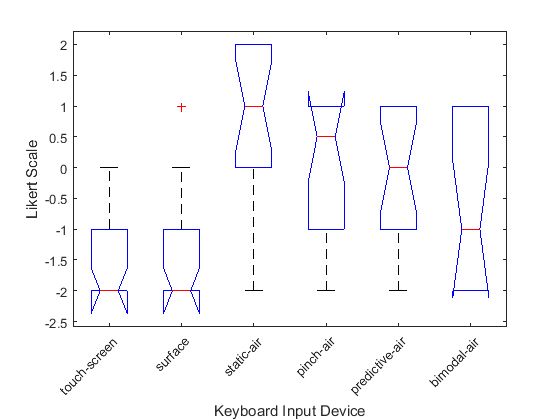
\includegraphics{Figures/fig_fatigue_boxplot}
	\caption[Level of Fatigue Boxplot]{Median Level of Fatigue for each keyboard showing the 25th and 75th percentiles.}
	\label{fig_fatigue_boxplot}
\end{figure}

The multiple comparisons, seen in Table~\ref{fatigue_multcompare}, revealed significant differences ($p$-values $<$ 0.01) in Level of Fatigue between the Touch Screen Keyboard and the Leap Static-air, Pinch-air, and Predictive-air keyboards. There were significant differences ($p$-values $<$ 0.05) between the Leap Surface Keyboard and the Static-air, Pinch-air, and Predictive-air keyboards. There was also a significant difference ($p$-value $=$ 0.0043) found between the Leap Bimodal-air and the Static-air keyboards. As expected, the fatigue levels experienced for mid-air keyboards were typically higher than those that were not mid-air.

\subsection{Level of Difficulty}
%means = -1.7222   -1.4444   -0.2222   -0.6667   -0.6667   -1.2778
%stds = 0.5745    0.7048    1.1144    1.1882    1.2834    0.8264
Keyboards reached a median Level of Difficulty of ``Strongly Disagree'' for the Touch Screen Keyboard, ``Strongly Disagree'' for the Leap Surface Keyboard, between ``Disagree'' and ``Neutral'' for the Leap Static-air Keyboard, ``Disagree'' for the Leap Pinch-air Keyboard, ``Disagree'' for the Predictive-air Keyboard, and ``Disagree'' for the Leap Bimodal-air Keyboard. Figure~\ref{fig_difficulty_boxplot} shows the median Level of Difficulty for each keyboard interaction style rated by the participants. Using a one-way ANOVA, a significant difference was detected between keyboard means for Level of Discomfort ($F(5, 102) = 6.0351$, $p$-value $<$ 0.0001, $SD_{pooled} = 0.98$), prompting the use of Tukey's HSD with multiple-compare for further analysis.

\begin{figure}[!t]
	\centering
	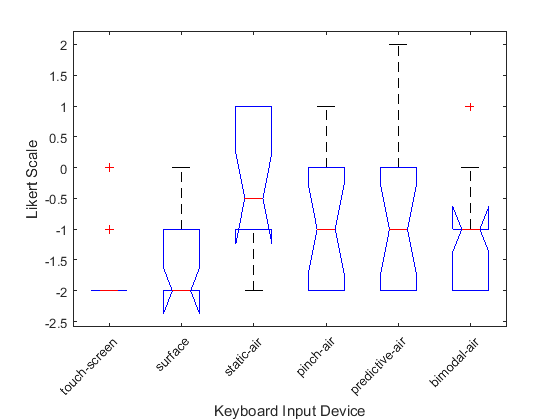
\includegraphics{Figures/fig_difficulty_boxplot}
	\caption[Level of Difficulty Boxplot]{Median Level of Difficulty for each keyboard showing the 25th and 75th percentiles.}
	\label{fig_difficulty_boxplot}
\end{figure}

The multiple comparisons, seen in Table~\ref{difficulty_multcompare}, revealed significant differences ($p$-values $<$ 0.05) in Level of Difficulty between the Touch Screen Keyboard and the Leap Static-air, Pinch-air, and Predictive-air keyboards. There was significant difference ($p$-values $=$ 0.0042) between the Leap Surface and the Static-air keyboards. There was also a significant difference ($p$-value $=$ 0.0209) found between the Leap Bimodal-air and the Static-air keyboards. As anticipated, the mid-air keyboards had a higher level of difficulty and were harder to use or understand than the non-mid-air keyboards.

\subsection{Preference Ranking}
Participants reached a mean Preference Ranking of 1.89 ($SD = 1.18$) for the Touch Screen Keyboard, 2.22 ($SD = 1.22$) for the Leap Surface Keyboard, 5.33 ($SD = 0.84$) for the Leap Static-air Keyboard, 4.22 ($SD = 1.06$) for the Leap Pinch-air Keyboard, 4.50 ($SD = 1.42$) for the Predictive-air Keyboard, and 2.83 ($SD = 1.29$) for the Leap Bimodal-air Keyboard. Figure~\ref{fig_ranking_mean} shows the mean Preference Ranking for each keyboard interaction style. Using Friedman's rank-test, ANOVA, a significant difference was detected between keyboard means, $\chi^{2}(5, 85) = 49.1429$, $p$-value $<$ 0.0001, $SD_{pooled} = 1.87$), prompting the use of Tukey's HSD with multiple-compare for further analysis.

\begin{figure}[!t]
	\centering
	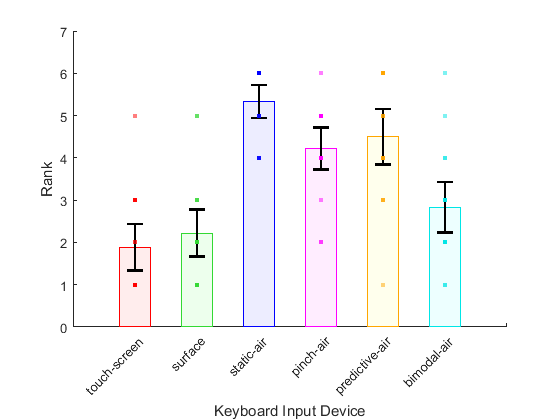
\includegraphics{Figures/fig_ranking_mean}
	\caption[Mean Preference Rankings]{Mean Preference Rankings for each keyboard with error bars showing 95\% confidence intervals.}
	\label{fig_ranking_mean}
\end{figure}

The multiple comparisons, seen in Table~\ref{ranking_multcompare}, revealed significant differences ($p$-values $<$ 0.01) in Preference Ranking between the Touch Screen Keyboard and the Leap Static-air, Pinch-air, and Predictive-air keyboards. There were significant differences ($p$-values $<$ 0.05) between the Leap Surface Keyboard and the Static-air, Pinch-air, and Predictive-air keyboards. There was also a significant difference ($p$-value $=$ 0.0009) found between the Leap Bimodal-air and the Static-air keyboards.

The preference ranking of all of the keyboards very strongly reflected the trends seen in most of the other dependent measures. The Touch Screen Keyboard was the most preferred, as expected, followed by the Leap Surface in a close second. The Leap Bimodal-air was the most preferred mid-air keyboard, whereas the Static-air Keyboard was the least preferred.